\documentclass[10pt,letterpaper]{article}
\usepackage[margin=0.88in]{geometry}
\usepackage[T1]{fontenc}
\usepackage{newtxtext,newtxmath}
\usepackage{microtype}
\usepackage{amsmath,booktabs,graphicx}
\usepackage{hyperref}
\hypersetup{colorlinks=true,urlcolor=blue,linkcolor=black,citecolor=black,pdftitle={Can Lagged Yield Changes Beat a Random Walk?},pdfauthor={Jonah Engelmann, Leo Gordon, Malcolm Siljehag Alencar}}
\usepackage{caption}
\usepackage{float}
\captionsetup{font=small,labelfont=bf}
\usepackage{enumitem}
\setlist[itemize]{nosep,leftmargin=2.2em}
\setlength{\parindent}{1.4em}
\setlength{\parskip}{2.0pt}
\setlength{\textfloatsep}{10pt}
\setlength{\intextsep}{8pt}
\newcommand{\bp}{\,\mathrm{bp}}
\newcommand{\RMSE}{\operatorname{RMSE}}
\title{\vspace{-2em}\textbf{Can Lagged Yield Changes Beat a Random Walk?}\\[2mm]
\large One-day forecasts for the 10-year U.S. Treasury yield}
\author{Jonah Engelmann \qquad Leo Gordon \qquad Malcolm Siljehag Alencar\\
\normalsize ESE 5420 --- Final Project Report}
\date{November 2026}
\begin{document}
\maketitle
\vspace{-1.25em}
\begin{abstract}
We study whether recent changes in the 10-year U.S. Treasury yield forecast the next daily change better than a random walk. Ordinary least squares (OLS) and $k$-nearest neighbors ($k$NN) are selected by expanding-window quarterly validation over 2021--2022 and evaluated on 2023 without refitting. The zero-change forecast achieves a 2023 root mean squared error (RMSE) of 7.461 basis points (bp), compared with 7.486 bp for OLS and 7.573 bp for $k$NN. Relative to zero change, the RMSE differences are 0.025 bp (95\% paired block-bootstrap interval [-0.018, 0.066]) and 0.112 bp ([0.018, 0.198]), respectively. OLS is not distinguishable from the zero-change forecast at this precision; $k$NN performs worse. Neither model yields an out-of-sample improvement.
\end{abstract}

\section{Question and data}
Let $r_t$ denote the 10-year U.S. Treasury par yield, quoted in percentage points on observation day $t$. We forecast the next observed daily change
\begin{equation}
    y_t=100(r_t-r_{t-1})\bp,
    \qquad x_t^{(p)}=(y_{t-1},\ldots,y_{t-p})^\top\in\mathbb R^p.
    \label{eq:features}
\end{equation}
One unit of $y_t$ is one basis point. In particular, $x_t^{(p)}$ is measurable before $r_t$ is observed. The question is whether either fitted model improves the \emph{2023} RMSE relative to the forecast $\widehat y_t=0$, by an amount larger than its sampling error.

We use the U.S. Treasury's \href{https://home.treasury.gov/resource-center/data-chart-center/interest-rates/daily-treasury-rate-archives/par-yield-curve-rates-2020-2023.csv}{daily par yield curve archive} for 2020--2023. We sort observations by date and difference successive observed trading days. The 1,001 records contain no duplicate dates or missing 10-year yields. Missing calendar days are not filled. Only the 10-year maturity is used; introducing other maturities would change the scope of the experiment.

\begin{table}[H]
\centering
\caption{Daily yield observations and realized zero-change RMSE. The first difference in 2020 is unavailable; subsequent years use the preceding year's last quote.}
\label{tab:data}
\begin{tabular}{lrrr}
\toprule
Year & Yield observations & Yield changes & Zero-change RMSE (bp)\\
\midrule
2020 & 251 & 250 & 5.504\\
2021 & 251 & 251 & 4.277\\
2022 & 249 & 249 & 7.828\\
2023 & 250 & 250 & 7.461\\
\bottomrule
\end{tabular}
\end{table}

\section{Models and evaluation protocol}
The zero-change forecast, $\widehat y_t^{(0)}=0$, is a random walk in yield levels, $\widehat r_t=r_{t-1}$. We compare it with two fitted one-step forecasts using exactly the features in \eqref{eq:features}:
\begin{align}
\text{Linear:}\quad &\widehat y_t=\widehat\beta_0+\widehat\beta^\top x_t^{(p)},\\
\text{$k$NN:}\quad &\widehat y_t=\frac1k\sum_{i\in\mathcal N_k(x_t^{(p)})}y_i.
\end{align}
The linear model is ordinary least squares with an intercept. For $k$NN we standardize each feature using the current training window's mean and standard deviation, then use Euclidean distance and uniform neighbor weights. The standardization is refitted whenever the training window expands.

We choose $p\in\{1,2,3,4,5\}$ for each model and $k\in\{3,5,10,20,40\}$ for $k$NN. For each candidate, we fit on all available observations strictly before the validation quarter and predict that next quarter; the eight validation quarters run from 2021 Q1 to 2022 Q4. The selection criterion is the \emph{mean of the eight quarterly RMSEs}. Their sample standard deviation describes the variation across quarters. We then refit the selected model once on 2020--2022 and make one-step-ahead forecasts throughout 2023, with fixed coefficients or training neighbors. A 2023 forecast may use realized earlier 2023 changes as lags, but never to refit the model or its scaler.

For model $m$, we report
\begin{equation}
\RMSE_m=\sqrt{\frac1n\sum_{t=1}^n(y_t-\widehat y_{m,t})^2},\qquad
D_m=\RMSE_m-\RMSE_0.
\label{eq:delta}
\end{equation}
Negative $D_m$ favors the fitted model. We estimate uncertainty in $D_m$ with a paired circular moving-block bootstrap of the 250 test dates: sample contiguous blocks of 20 observations with replacement, concatenate and truncate to 250 dates, and recompute both RMSEs on the same indices. We use 10,000 replications and percentile 95\% intervals. The interval measures uncertainty conditional on the fitted forecasts and does not account for hyperparameter-selection uncertainty.

\section{Results}
\subsection{Expanding-window validation}
\begin{table}[H]
\centering
\caption{Validation RMSE across eight quarters, in bp. The mean is used for selection; $\pm$ reports the sample standard deviation of quarterly RMSEs. The same validation periods are used for all rows.}
\label{tab:cv}
\begin{tabular}{lcc}
\toprule
Forecast & Lags / neighbors & Mean $\pm$ s.d. (bp)\\
\midrule
Zero change & --- & 6.028 $\pm$ 1.993\\
OLS & $p=1$ & 6.052 $\pm$ 1.963\\
OLS & $p=2$ & 6.068 $\pm$ 1.922\\
OLS & $p=3$ & 6.079 $\pm$ 1.955\\
OLS & $p=4$ & 6.087 $\pm$ 1.957\\
OLS & $p=5$ & 6.113 $\pm$ 1.952\\
$k$NN (best) & $p=2,\ k=40$ & 6.059 $\pm$ 1.946\\
\bottomrule
\end{tabular}
\end{table}

The lowest validation error for the linear model occurs at $p=1$. For $k$NN, the chosen configuration is $p=2$ and $k=40$. The differences between the leading candidates and the zero forecast are small relative to quarter-to-quarter variation. Figure~\ref{fig:cv} shows that the error level changes more across quarters than across the models.

\begin{figure}[H]
\centering
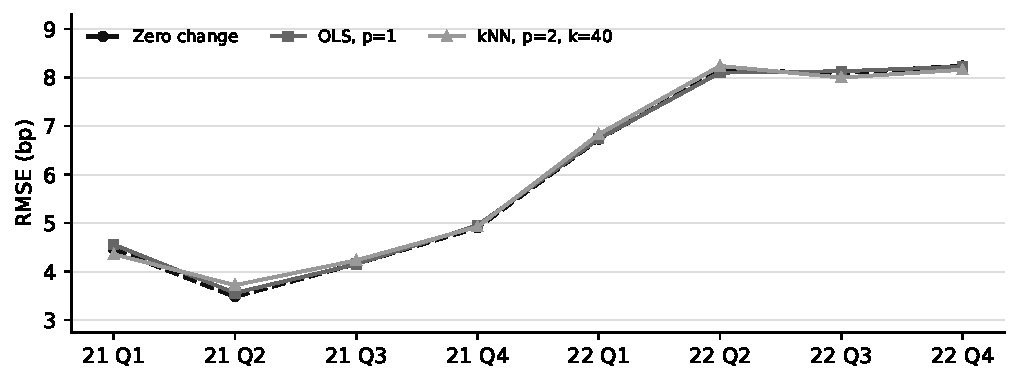
\includegraphics[width=.72\linewidth]{validation_rmse.pdf}
\caption{Quarterly validation RMSE. Each model is fitted using only days before the corresponding quarter; the displayed OLS and $k$NN configurations are the winners of the validation search.}
\label{fig:cv}
\end{figure}

\subsection{2023 held-out comparison}
\begin{table}[H]
\centering
\caption{Held-out 2023 forecasts ($n=250$). $D$ is fitted-model RMSE minus zero-change RMSE; a negative value means improvement. The intervals use paired 20-day bootstrap blocks.}
\label{tab:test}
\begin{tabular}{lrrl}
\toprule
Forecast & RMSE (bp) & $D$ (bp) & 95\% interval for $D$ (bp)\\
\midrule
Zero change & 7.461 & --- & ---\\
OLS ($p=1$) & 7.486 & 0.025 & [-0.018, 0.066]\\
$k$NN ($p=2,k=40$) & 7.573 & 0.112 & [0.018, 0.198]\\
\bottomrule
\end{tabular}
\end{table}

The linear model's difference is 0.025 bp; its interval includes zero. On this test year, we cannot distinguish its predictive error from that of the zero-change forecast at the stated precision. $k$NN's difference is positive, and its interval lies above zero. Neither model beats the random walk. With 10- or 30-day bootstrap blocks, the intervals remain consistent with the same conclusion: OLS ([-0.017, 0.064] and [-0.014, 0.066] bp); $k$NN ([0.018, 0.201] and [0.014, 0.203] bp).

\section{Discussion}
Recent 10-year yield changes provide little one-step predictive information under either fitted model. Validation RMSEs are close to the zero-change benchmark, whereas the level of forecast error varies substantially over time: the benchmark RMSE rises from 4.277 bp in 2021 to 7.828 bp in 2022. These results concern a narrow information set, not predictability from the yield curve or other market variables more broadly.

The test covers one calendar year. Paired block-bootstrap intervals account for serial dependence in the observed forecast errors, conditional on the fitted models, but cannot establish performance across different interest-rate regimes. The Treasury's longer archive begins in 1990, providing a basis for experiments with larger training samples.

\paragraph{Extensions.}
One extension is to include lagged 2-year and 30-year changes, the previous day's 2s10s and 10s30s spreads, and rolling volatility. These variables would test whether cross-maturity interactions or the recent scale of rate movements help forecast the conditional mean. A nonlinear tabular model such as TabPFN-3.5 (J\"ager et al., 2026) provides a useful comparison with OLS and $k$NN. Because the 2023 results are already observed, such a comparison would need model selection on earlier chronological windows and a new, untouched test period, for example 2024--2025. This separates information gained from richer features from that gained through a more flexible model.

\paragraph{Reproducibility.}
The analysis uses the dated Treasury CSV, eight expanding-window validation quarters, and 10,000 paired circular moving-block bootstrap replications with 20-day blocks (random seed 5420). Source code, data, and the validation figure accompany the report.

\section*{References}
\noindent U.S. Department of the Treasury. \emph{Daily Treasury Par Yield Curve Rates: 2020--2023}. \href{https://home.treasury.gov/resource-center/data-chart-center/interest-rates/daily-treasury-rate-archives/par-yield-curve-rates-2020-2023.csv}{Data archive}.\\
\noindent U.S. Department of the Treasury. \emph{Interest Rates Data CSV Archive}. \href{https://home.treasury.gov/interest-rates-data-csv-archive/}{Historical series}.\\
\noindent K\"unsch, H. R. (1989). The jackknife and the bootstrap for general stationary observations. \emph{The Annals of Statistics}, 17(3), 1217--1241.\\
\noindent J\"ager, B., et al. (2026). \emph{TabPFN-3.5: Technical Report}. \href{https://arxiv.org/abs/2609.17895}{arXiv:2609.17895}.

\end{document}
